\documentclass[11pt]{article}
%\documentstyle[11pt]{article}
\usepackage{hyperref}
\usepackage{color}
\usepackage{epsf}
\usepackage{natbib}
\usepackage{graphicx}
%%
%%   Edition of 2017.03.16_22:07:26
%% 
\input mace.tex
\newcommand{\pid}   {\par\hangindent=2em\hangafter=-9\noindent}
\newcommand{\ppid}  {\par\hangindent=4em\hangafter=-9\noindent}
\newcommand{\pppid} {\par\hangindent=6em\hangafter=-9\noindent}
\newcommand{\ppppid}{\par\hangindent=8em\hangafter=-9\noindent}
%\newcommand{\nthr}[1]{ \multicolumn{3}{ @{} l }{#1} }
\renewcommand{\epsilon}{\varepsilon}
\renewcommand{\phi}{\varphi}
%\newcommand{\dss}{\displaystyle}
\newcommand{\dint}{\int\hspace{-0.25em}\int}
\newcommand{\sinc}{\rm sinc }
\newcommand{\hh}{\hphantom}
\newcommand{\hp}{\hphantom{+}}
\newcommand{\vi}{\vphantom{\int}}
\renewcommand{\hm}{\hphantom{-}}
\newcommand{\vex}{\vspace{1ex}}
\newcommand{\den}{\Frac{1}{c}\Frac{1}{1 + \Frac{1}{c}\lp \vec{V_{\earth}}(t_1)\, + \dmat{E}(e(t_1))\,\vec{r}_2\rp} }
\definecolor{Dred}{rgb}{0.312,0.070,0.070}
\definecolor{Dblue}{rgb}{0.070,0.070,0.312}
\definecolor{Dgreen}{rgb}{0.070,0.312,0.070}
\definecolor{Db}{rgb}    {0.050,0.0,0.320}
\newcommand{\Grb}[1]{\textcolor{Dgreen}{\bf #1}}
\newcommand{\Blb}[1]{\textcolor{Dblue}{\bf #1}}
\newcommand{\Rdb}[1]{\textcolor{Dred}{\bf #1}}
\definecolor{LightSiren}{rgb}{0.941,0.921,0.972} 
\definecolor{LightGreen}{rgb}{0.941,0.972,0.921}
\newcommand{\hurl}[1]{\textcolor{Db}{\bf http:/$\!$/#1}}
\newcommand{\furl}[1]{\textcolor{Db}{\bf ftp:/$\!$/#1}}
\newcommand{\Gr}[1]{\textcolor{Dgreen}{\bf #1}}
\newcommand{\Or}[1]{\textcolor{Dorange}{\bf #1}}
\newcommand{\Rd}[1]{\textcolor{Dred}{\bf #1}}
\newcommand{\Bl}[1]{\textcolor{Dblue}{\bf #1}}
\newcommand{\web}[1]{\Blb{\url{#1}}}
\newcommand{\PIMA}{\textcolor{Dgreen}{$\cal P\hspace{-0.067em}I\hspace{-0.067em}M\hspace{-0.067em}A$} }
\renewcommand{\topfraction}{0.95}
\renewcommand{\textfraction}{0.05}

\voffset    = -30mm
\hoffset    = -15mm
\textwidth  = 165mm
\textheight = 235mm
\tolerance  = 600
\hfuzz      = 0.3mm

\title {  \LARGE\bf Memo: On normalization of visibility amplitudes in VLBI processing}
\author{ {\large\sc L. Petrov} \\
         {\small Leonid.Petrov@lpetrov.net }
       }
\date{2017.03.16}

\begin{document}

\maketitle

\section{Amplitude normalization}

  The raw fringe amplitude has a number of biases. First bias is due to 
digitization. A general theory of digitization correction is developed
by \citet{r:kog98}. For a case of small amplitudes, i.e cross-correlation,
the digitization correction on does not on the amplitude and is reduced to 
scaling: for a case of two-bit digitization the raw fringe amplitude
has to be divided by 0.8825, for the case of 1-bit sampling has to be 
divided by 0.6366, and for a case of mixed 1-bit/2-bit sampling when 
one station records 2-bit and another records 1-bit the amplitude has
to by divided by the scaling factor of 0.7495 in order to compensate 
distortion caused by digitization.

  Digital correction of the autocorrelation is more complicated for two 
reasons. Firstly, for a case of large amplitudes the digital correction
depends on amplitude and its functional dependence is not described by
a simple scaling law. Secondly, the digital correction is defined for 
the correlation coefficient, not for the visibility spectrum, which
is the Fourier transform of the lagged correlation. In order to perform
digital correction of autocorrelation data, we do the following steps:
%
\begin{itemize}
    \item put autocorrelation data in [1,N] part of the array
          sized [1,2N], where $N$ is the number of spectral channel
          in a given IF;

    \item compute autocorrelation at point N+1 by linear extrapolation:
          A[N+1] = 2*A[N] - A[N-1];

    \item pad the remaining part of the extended autocorrelation array 
          to zero: A[N+2:2N] = 0.0;

    \item perform Fourier transform of the extended autocorrelation 
          array of dimension 2N and divide it by 2N for proper
          normalization: $a = {\cal F}(A)/(2N)$. Since the input
          autocorrelation is Hermitian, the output will have N+1
          non-zero elements.

    \item compute the autoconvolution of the rectangular taper as
          $T(i) = 1 - (i-1)/N$;

    \item normalize autocorrelation to 1 at zero lag: $T_n = a(1)$

    \item de-taper and normalize Fourier transform of the autocorrelation:
          $a_n[i] = a[i]/(T_n*T[i])$, which gives are the autocorrelation
          coefficient in lag domain;

    \item apply digital correction to the autocorrelation coefficient
          using tables computed by \citet{r:kog_mem5}:
          $a_d[i] = D(a_n[i])$ for $i=1,2, \ldots N+1$;
          
    \item Add symmetrical values of the lag correlation function in order
          to get real autocorrelation spectrum:
          $a_d[i] = a_d[2N+2-i]$ for $i=N+2,N+3, \ldots 2N$;

    \item Perform inverse Fourier transform of $a_d[i]$, which provides
          us the autocorrelation corrected for distortion due to digitization.
\end{itemize}

  The explanation of the algorithm can by found in \citep{r:kog_mem6}.
             
  The correlator may also have biases in fringe amplitude. In order to
calibrate for biases common for autocorrelation and cross-correlation, we
compute average of autocorrelation amplitude over the IF bandwidth. For the 
perfect hardware and correlator this average value should be 1.0 according
to Parseval theorem. It can deviate from 1.0 for several reasons. 
If the amplitude level of 2-bit sampling deviates from the optimal level,
the 2-bit digitization correlation deviates from 0.8825. Old VLBA hardware 
correlator had a weird factor of 0.9028 for 1-1 bit sampling, 1.6834
for 2-2 bit sampling and 1.2347 for 1-2 bit sampling \citep{r:kog_mem12}.
The origin of these factors is lost\footnote{I asked in 2013 Leonid Kogan who
derived these factors what is their origin and he replied firmly: ``I do not
remember''.}. The DiFX software correlator does not have these factors 
intrinsically, but it scales the visibility data by them to have raw amplitude 
as close as possible to the old hardware VLBA correlator. The SFXC software
correlator does not apply these factors.

  In order to correct visibility for scaling factors common for autocorrelation
and cross correlation we divide cross-correlations by 
$\sqrt{\bar{A}_i \cdot \bar{A}_j}$, where $\bar{A}_i$ is the mean 
autocorrelation corrected for digitization distortion averaged over both 
frequency and time. {\bf NB:} even if we mask out a portion of the bandwidth, 
we average autocorrelation over the entire bandwidth regardless of mask.

  There is a caveat related to the old  VLBA hardware correlator. It was 
found that for high amplitudes (autocorrelation case), the internal correlator 
registers saturate. This saturation decreases the accumulated amplitude due to 
limited number of bits in the digital representation of the amplitude. Though,
the saturation effect is negligible in cross correlation. The saturation is 
1 + $w$/8 for single polarization data and 1 + $w$/4 for dual polarization 
data, were $w$ the data weight defined as the ratio of the number of bits used 
to the total number of bits recorded. Since the saturation decreases the 
autocorrelation amplitude and since we have divided the cross-correlation 
amplitude by $\sqrt{\bar{A}_i \cdot \bar{A}_j}$, we need divide 
cross-correlation amplitude by the saturation factors in order to compensate 
cross-correlation amplitude.

  The input FITS-IDI files have a field ``CORRELAT'' that supposed to designate
the correlator. Unfortunately, this field is not always populated, so \PIMA\ 
may not know which correlator generated the data. \PIMA\ has keyword
\Blb{FRIB.AMPL\_FUDGE\_TYPE} that specifies the correlator name directly
(for instance DIFX or VLBA (for hardware correlator)). \PIMA\ supports 
a variant of saturation calibration \Blb{VLBA\_KOGAN} that 1 + 1/8 
for single polarization data and 1 + 1/4 for dual polarization data, i.e.
considering that weights do not affect the saturation calibration. 
It remains obscure which flavor of saturation calibration is better.

\section{Bandpass computation}

   We consider that observed visibility $V_{\rm 12,obs}$ is related to
the true visibility $V_{12}$ with the ideal hardware as
%
\beq
   V_{\rm 12,obs}(f) = V_{\rm 12, ideal}(f) \: B_1^{*}(f) \cdot B_2(f)
\eeq{e:e1}

  where $B_i$ is a complex station-dependent function that describes
distortion of the signal in the VLBI hardware\footnote{This definition 
describes the amplitude response to voltage. AIPS has the same convention.
Alternatively one can define bandpass as the amplitude response 
to power.} Typically, the amplitude response at a baseline is a tooth-like. 

  There are two factors that determine the amplitude response. First, 
the amplitude response of an individual IF to a signal with a flat spectrum
distorts the input signal and makes its spectrum non-flat. The autocorrelation
spectrum describes the spectrum of a flat spectrum signal that passes through
the VLBI hardware. Secondly, a signal at a given IF has an admixture of the 
signal from adjacent IFs, mainly at the edges of the IF band (see 
illustrations in the Appendix). This leaked signal is not coherent and causes 
decorrelation. Decorrelation is a function of frequency: it is greater at 
the edge of the IF. Therefore, a cross-correlation bandpass 
$B_1^{*}(f) \cdot B_2(f)$ in general is not equal to the product of 
autocorrelation bandpasses $\sqrt{A_1(f) \cdot A_2(f)}$.

  The bandpass can be determined from observations of strong sources
with continuum spectrum. We can neglect changes of the flux density
over the intermediate frequency (IF) bandwidth and consider the spectrum
flat, i.e frequency-independent.  In that case the product of voltage 
bandpasses $B_1^{*}(f) \cdot B_2(f)$ is just the normalized cross-spectrum
of the calibrator spectrum $\frac{1}{n} V_{\rm 12,obs}(f)$, where 
$n$ is the normalization coefficient.

  \PIMA\ determines bandpass at a given polarization in three steps.
At the first, so-called {\sc init} step, \PIMA\ examines results of the
coarse fringe search and finds the observations with the greatest
SNR at each baseline with the reference station. Initially, the so-called
power baseline bandpass 
$B_{\rm ir,bas} = \frac{1}{n_{\rm bas}} V_{\rm ir,obs}(f)$
is computed, where the normalization factor over the total IF band is
%
\beq
   n_{\rm pow}(B,f_l,f_h) = \Frac{\int\limits_{f_l}^{f_h} |B(f)|  \, df}
                                 {f_h - f_l},
\eeq{e:e2}
%
where, $f_l$ and $f_h$ are the lower and upper frequencies of the
IF, i.e. we require the normalized bandpass to have unity integral over
the IF bandwidth. The visibility $V_{\rm ir,obs}(f)$ used for bandpass 
computation are phase rotated with results of fringe fitting and averaged 
over time:
%
\beq
   V_{\rm ir,obs}(f) = \dss\sum\limits_{k} \sum\limits_{j} v_k(f_j,t) 
             e^{2\pi \, (  f_0 \tau_p \; + \;
                           f_0 \dot{\tau}_p (t_k - t_0) \; + \;
                           (f_j - f_0) \tau_g \; + \;
                           (f_j - f_0) \dot{\tau}_g (t_k - t_0) )},
\eeq{e:e3}
%
 where $v_k$ is the raw visibility, $\tau_p$ is phase delay, $\tau_g$ is group
delay, $\dot{\tau}_p$ and $\dot{\tau}_g$ are their time derivatives, $f_0$
and $t_0$ are the reference frequency and fringe reference time respectively.
if the schedule had strong sources with SNR $>$ 100, usually there is not need
to average over frequency. If by oversight the schedule did not have strong 
sources, the IF is split into segments, and visibilities are coherently 
averaged over segments. The number of spectral channels within a segment is 
controlled by parameter \Blb{BPS.MSEG\_ACCUM}. Value 1 means that no 
averaging is to be performed.

Since even for sources with the SNR $>$ 1000 the visibility spectrum 
$V_{\rm ir,obs}(f)$ has a noticeable scatter, \PIMA\ smooths it with
either using Legendre polynomial (\Blb{BPS.INTRP\_METHOD: LEGENDRE})
or smoothing B-spline of the 3rd degree (\Blb{BPS.INTRP\_METHOD: SPLINE}). 
Parameters\Blb{BPS.DEG\_AMP} and \Blb{BPS.DEG\_PHS} control the degree
of the Legendre polynomial or the number of knots for the smoothing 
B-spline. When processing $V_{\rm ir,obs}(f)$ phase, \PIMA\ performs 
phase ambiguities resolution. Normalization is performed after 
smoothing.

  Then the bandpass of the reference station is computed as
%
\beq
   B_r(f) = \frac{1}{n_{\rm pow}}(B,f_l,f_h) \lp 
           \prod \limits_{i}^{n-1} |B_{\rm ir,bas}| \rp^{\frac{1}{2(n-1)}}
\eeq{e:e4}
%
where normalization is computed the same was as in equation~\ref{e:e2}.
The bandpass of the reference stations is set to the geometric mean
of the bandpasses of all remote stations. Its phase is set to zero.

  After we found the bandpass of the reference station, we compute 
voltage bandpasses from power bandpasses: 
$B_{\rm ir} = \frac{1}{n_{\rm vol}} (B_r,f_l,f_h)
                                     B_{\rm ir,bas}/B_r{f}$.
Voltage bandpass is normalized differently: 
%
\beq
   n_{\rm vol}(B_i,B_r,f_l,f_h) = 
        \Frac{ \int\limits_{f_l}^{f_h} 
               \sqrt{|B_i(f)| \cdot |B_r(f)| } \, df}
             {f_h - f_l},
\eeq{e:e5}
%
i.e. we require the square root of power of the product of the 
bandpasses at a given station and the reference station to have 
the integral over the IF bandwidth equal to unity.
  
  The second step is computation of the bandpass in the so-called 
{\sc accumulative} mode. First, \PIMA\ finds the list of $N$ observations
with the highest SNR for each baseline with the references station.
Parameter $N$ is defined in parameter \Blb{BPS.NOBS\_ACCUM} and does
not count the observation used in the {\sc init} mode. Fringe fitting 
for these observations is repeated and the phase bandpass computed
in the {\sc init} mode is applied to the observations before fringe 
fitting and the amplitude bandpass is applied after the fringe fitting. 
Expression ``apply bandpass'' means the visibilities of an observation 
are divided by the bandpass. Expression ``apply phase bandpass'' means 
the visibilities are divided by $B^{*}_1 \cdot B_2/(|B_1| \; |B_2|)$ 
and expression ``apply amplitude bandpass'' means the visibilities are 
divided by $|B_1| \; |B_2|$. Since we divide raw amplitudes by the 
product ot amplitude bandpasses, this explains why we normalize the
bandpasses at individual stations to the square root of power.
It should be noted that the amplitude bandpass should never be applied 
before fringe fitting. Applying the amplitude bandpass before fringe 
fitting would have resulted to up-weighting visibilities at frequencies 
where the bandpass is small, i.e. at the edges of the bandwidth. Such 
up-weighting would have decreased the SNR.

  After running fringe fitting in the accumulative mode, \PIMA\ computes
residual time-averaged complex visibilities normalized over (i.e. divided 
by) time and frequency. Had the bandpass been absolutely stable in time, 
the residual spectrum presented as a complex number would be (1.0, 0.0). 
\PIMA\ computes the arithmetic average phase of normalized residuals $R$
as $\Psi(f) = \sum R_i(f)/|R_i(f)|/n$ and geometric average of their 
amplitudes as $\kappa(f) = \prod |R_i(f)|^{1/n}$ and computes phase and 
amplitude of accumulative bandpass as $\Psi(f)$ and 
$ 1/n_{\rm vol}(B_i,B_r,f_l,f_h) \: \kappa(f)/|B_r(f)|$ respectively. The
amplitude of the stacked residual amplitude bandpass is divided by the 
amplitude of the {\sc init} bandpass of the reference station and, thus,
is transformed to the voltage bandpass. The bandpass of the reference 
station is not updated at this step.

  The third step is computation of the bandpass in the so-called 
{\sc fine} mode using least squares. First, \PIMA\ finds the list of $K$ 
observations with the highest SNR for each baseline with the references 
station. Parameter $K$ is defined by keyword \Blb{BPS.NOBS\_FINE} and 
includes the observation used in the {\sc init} mode. Similar to the 
previous step, the phase bandpass computed in the accumulative mode is 
applied before fringe fitting, the amplitude bandpass is applied after 
fringe fitting, and the normalized complex residuals $R(f)$ averaged 
over time are computed. Then the coefficients of the bandpass expansion 
for all stations are computed in a single least square solution. 
The phase bandpass is computed as
%
\beq
    \sum b_{ir} P_j(f) = \Frac{R_{ir}(f)}{|R_{ir}(f)|}.
\eeq{e:e6}
%
where $b_{ij}$ are the coefficients for the $i$-th station and $P_j(f)$
is the basic function. The amplitude bandpass is computed as
%
\beq
    \sum a_{i} P_j(f) + a_{r} P_j(f) = \log |R_{ir}(f)|.
\eeq{e:e7}

  Here $a_{ij}$ are the coefficients of expansion of the bandpass logarithm
for stations with index $i$ and~$r$. After computation of the bandpass in 
{\sc fine} mode, \PIMA\ computes residuals after applying this bandpass 
and identifies the observations with the largest root mean square phase 
residuals and the observations and the largest root mean square amplitude 
residuals. If the residuals exceed the limits specified by parameters 
\Blb{BPS.PHAS\_REJECT} and \Blb{BPS.AMPL\_REJECT}, \PIMA\ removes such 
an observation from the bandpass computation and updates the least square 
solution. The iterations are performed till either the rms of residuals 
becomes less than \Blb{BPS.PHAS\_REJECT} and \Blb{BPS.AMPL\_REJECT}, or 
the number of remaining observation at a given baseline becomes
\Blb{BPS.MINOBS\_FINE}.

  The final bandpasses for all stations but the reference one are 
renormalized once again using voltage renormalization.

  The main reason why a three-step procedure is implemented in \PIMA\ is to
detect and mitigate the influence of bad observations on bandpass computation.
It is not uncommon when observations with the largest SNR are affected
by the radio interference (RFI). If only one observation is used for 
bandpass computation at a given baseline, i.e. bandpass computation is 
limited to the {\sc init} mode, and that observation is affected by RFI, 
the bandpass will be suitable only for that observation, and all other 
observations will become affected by the influence of the RFI when corrupted 
bandpass is applied. Bandpass computation in the {\sc accumulative} mode 
allows to dilute the influence of bad observations. Bandpass computation in 
the {\sc fine} mode allows to remove several bad observations from bandpass 
computation automatically mode and completely eliminate their influence. 
The three-step procedure also mitigates possible bandpass computation failures
due to incorrectly resolved phase ambiguities. Phase ambiguities need be 
resolved only when processing the first observation in the {\sc init} mode. 
All other steps use visibilities with applied phase bandpass, and the 
residual phases are supposed to be much smaller than 1/2 phase turn.

  It is important to examine logs of bandpass computation. Statistics
of residuals of bandpass computation allows us to make a judgment how stable 
the bandpass is over time. It may happen that due to a hardware reset 
bandpass at one or more stations is different for a portions of the 
experiment. At the moment, \PIMA\ does not provide a convenient tool for 
processing observations with jumps in bandpasses. Processing such 
observations requires splitting the dataset into segments with stable 
bandpass and computing the bandpass for the segments separately.

  I would like to emphasize that one of the most important part of VLBI 
data analysis is to compute a precise phase and amplitude bandpass. 
{\bf It is a waste of time to process VLBI data with a poor bandpass!}

\section{Bandpass renormalization}

  \PIMA\ applies voltage normalization for bandpass. That normalization
preserves the sum of amplitudes over frequency before and after applying 
the bandpass. This choice seems natural since it does not depend on 
specific knowledge of the hardware. However, this ``natural'' choice
is often results in a bias. Two factors attenuate cross-correlation 
amplitude at the IF edges: the IF filter and the presence of signal 
from adjacent IFs that is not coherent. The central part of a bandpass 
is usually not affected. \PIMA\ allows to specify the range of the 
bandwidth as representative and preforms renormalization. \PIMA\ performs 
renormalization when it runs \Blb{\it splt} task. Keyword 
\Blb{SPLT.BPASS\_NRML\_METHOD} specifies whether to  run renormalization
and specifies \Blb{SPLT.BPASS\_NRML\_RANGE} the range of representative
bandwidth as a fraction of the total bandwidth. \Blb{0.20:0.85} is 
a good choice for processing VLBA data with {\sf rdbe\_pfb} digital
filter setup. New normalization is computed as  
%
\beq
   n_{\rm ren}(B_i,B_r,f_l,f_h) = 
        \Frac{\int\limits_{f_l}^{f_h} \; M_i \; M_r \: 
                            \sqrt{ |B_i(f)| \cdot |B_r(f)|} \, df}
             {\int\limits_{f_l}^{f_h} \; M_i \; M_r\, df},
\eeq{e:e8}
%
  where $M_i$ and $M_r$ are so-called fringe masks, i.e. masks used during
fringe fitting. This choice of renormalization preserves the sum of amplitudes 
over frequency before and after applying the bandpass within the representative
portion of the bandwidth, excluding the spectral channels that are masked out.

  \PIMA\ supports four masks: autocorrelation mask, bandpass mask,
fringe mask and split mask. Fringe mask is applied during fringe fitting,
except task \Blb{\it bpas}. Task \Blb{\it bpas} uses the bandpass mask for 
fringe fitting. Task \Blb{\it splt} uses split mask for computing time and 
frequency averaged visibilities. It is important to emphasize that just 
fringe mask is to be used for bandpass renormalization.

  Applying bandpass renormalization usually results in an increase of image 
flux density. Such bandpass renormalization mitigates amplitude reduction 
due to decorrelation at the edges of the bandpass. Though, as 
Figures~\ref{f:vlba}--\ref{f:cvn} show, the choice of the representative
portion of the bandwidth is at some extent subjective. The subjectiveness
in the selection of the representative portion of the bandpass may result
in up-scaling or down-scaling flux densities at a level of several pro cents.

\section{Polarization bandpass}

  \PIMA\ supports so-called polarization bandpass $P_i(f)$ that is defined 
this way:

\beq
  \begin{array}{lcl}
     V^{RR}_{\rm 12,obs}(f) & = & V^{RR}_{\rm 12, ideal}(f) \: 
                                  B_1^{*}(f) \cdot B_2(f) \vex \\
     V^{LL}_{\rm 12,obs}(f) & = & V^{LL}_{\rm 12, ideal}(f) \: 
                                  B_1^{*}(f) \cdot B_2(f) \; 
                                  P_1^{*}(f) \cdot P_2(f) \cdot
                                  e^{2 \, i \, (\psi_1(t) - \psi_2(t))},
  \end{array}
\eeq{e:e9}
%
   where $\psi_i(t)$ is the feed horn rotation angle at the $i$-th station
with respect to the local meridian. Using other language, the polarization
bandpass is the averaged ratio of the spectrum of complex visibilities at 
LL polarization to the complex visibilities at RR polarization with phases 
corrected for the feed horn rotation.

   When dual-band data are processed, \PIMA\ treats RR data as the 1st 
polarization. It computes single-band RR bandpass using the procedure 
outlined above. When dual band are processed and keyword 
\Blb{POLARCAL\_FILE} is not set to \Blb{NO}, \PIMA\ for each step,
{\sc init}, {\sc accum}, {\sc fine} computes the corresponding polarization 
bandpass using the same observations as for RR bandpass. Thus, if 
\Blb{POLARCAL\_FILE} is not set to \Blb{NO}, \PIMA\ computes two bandpasses.

  In the {\sc init} mode \PIMA\ first applies the RR {\sc init} bandpass 
to RR data, computes residual spectrum $R^{RR}(f)$, then applies RR-bandpass 
to LL data, multiples visibilities by $e^{2 \, i \, (\psi_1(t) - \psi_2(t))}$
to compensate the differences in the contribution of the feed-horn rotation
angle to RR and LL visibilities and computes LL polarization residual spectrum
$R^{LL}$. Then $P_{\rm ir,raw} = R^{LL}/R^{RR}$. Then raw polarization bandpass
is smoothed with Legendre polynomials or B-splines, transformed from power
bandpass to voltage bandpass, and normalized the same way as RR-bandpass.

  In the {\sc init} mode \PIMA\ applies the {\sc init} polarization bandpass to 
LL-band residuals and get accumulative residuals:
$P_{\rm ir,acc}(f) = R^{LL}(f)/R^{RR}(f)/(P_i^{*}(f) \cdot P_r(f))$.
These accumulative residuals are averaged out, as an arithmetic mean for 
phase part and as a geometric mean for the amplitude part. The same voltage
normalization is applied for the polarization bandpass as for the RR single
polarization bandpass.
  
  In the {\sc fine} mode \PIMA\ applies the {\sc accum} polarization bandpass 
to LL-band residuals and get fine residuals. The parameters of the Legendre
polynomial and or B-spline expansion coefficients for phase of the polarization 
bandpass for all stations, except the reference one and the parameters of 
the polynomial or B-spline expansion coefficients for logarithm of the 
amplitude polarization bandpass are evaluated with a single least square
solution followed by identification the observations with the largest residual
and their removal from the parameter estimation process.

  Polarization bandpass allows to compute I-polarization visibilities on 
the fly before fringe fitting:
%
\beq
     V^{I}_{\rm 12}(f) & = & \Frac{1}{2}
         \Frac{V^{RR}_{\rm 12(f)} + 
               \Frac{V^{LL}_{\rm 12(f)} \; 
                     e^{2 \, i \, (\psi_1(t) - \psi_2(t))}
                    }
                    {\frac{P_1^{*}(f)}{|P_1(f)|} \cdot \frac{P_2(f)}{|P_2(f)|}
                    }
               }
               {\frac{B_1^{*}(f)}{|B_1(f)|} \cdot 
                \frac{B_2(f)}{|B_2(f)|}
               }.
\eeq{e:e10}

  I-polarization visibilities have approximately $\sqrt{2}$ higher SNR than
RR or LL visibilities\footnote{If amplitudes  of RR and LL visibilities 
are very close to each other than the advantage is exactly $\sqrt{2}$.},
which makes them attractive for detection of weak sources. A general 
recommendation is always to use I-polarization combination of dual-polarization
observables for fine fringe fitting. However, using I-polarization requires
a correctly computed polarization bandpass.

  Polarization bandpass re-normalization is performed differently:
%
\beq
   n_{\rm ren}(B_i,B_r,f_l,f_h) = 
        \Frac{\int\limits_{f_l}^{f_h} \; M_i \; M_r \: 
                          \sqrt{ |B_i(f)| \cdot |B_r(f)| \cdot 
                                 |P_i(f)| \cdot |P_r(f)|       } \, df}
             {\int\limits_{f_l}^{f_h} \; M_i \; M_r\, df},
\eeq{e:e11}
%
  
  Keyword \Blb{SPLT.POLAR} visibility for which polarizations should be
written in the output file. When \Blb{SPLT.POLAR: I} \PIMA\ task
\Blb{\it splt} calibrates visibilities for all four polarizations:

\beq
    \begin{array}{lcl}
       V^{RR}_{12} & = & \Frac{V^{RR}_{12}}{B^{*}_1 \cdot B_2}      \vex \\
       V^{LL}_{12} & = & \Frac{V^{LL}_{12} \: e^{2 \, i \, (\psi_1 - \psi_2)}}
                              {B^{*}_1 \cdot B_2 \cdot P^{*}_1 \cdot P_2} 
                                                                   \vex \\
       V^{RL}_{12} & = & \Frac{V^{RL}_{12} \: e^{-2 \, i \, \psi_2}}
                              {B^{*}_1 \cdot B_2 \cdot P_2} \;    \vex \\
       V^{LR}_{12} & = & \Frac{V^{LR}_{12} \: e^{ 2 \, i \, \psi_1} }
                              {B^{*}_1 \cdot B_2 \cdot P^{*}_1} \; 
                         
    \end{array}
\eeq{e:e12}

  \PIMA\ does not put I combination of RR and LL polarizations in the output;
it lets DIFMAP to generate such combinations. The feed horn rotation angle
is applied to left-circular polarization data to compensate the difference
in the sign of the feed horn rotation angle and is not applied to 
right-circular polarization data. So by convention, the polarization vector
of left-circular polarization data is aligned with the polarization
vector of right circular polarization data and both have the contribution
of the feed horn rotation angle with the sign that corresponds to the 
right-circular polarization visibilities.
  
\section{Autocorrelation renormalization}

  In VLBI data analysis we do not calibrate amplitude directly, but 
calibrate the noise level measured from the total power of the received 
signal that is the sum of the receiver thermal noise, atmospheric emission, 
Earth's surface emission that spills over to the receive, and the cosmological 
background radiation. The contribution from the observed source to the
total power is usually negligible. If we apply mask, and usually we do,
we cut some spectral channels. In general, the average power integrated 
over the used portion of the bandpass differs than the average power 
integrated over the entire IF bandwidth, since the IF bandpass is not 
rectangular. VLBI hardware always measures system temperature $T_{\rm sys}$ 
across the entire IF\footnote{Some VLBI data terminals measure $T_{\rm sys}$ 
across the entire band. At the moment, in such cases \PIMA\ assumes system 
temperature at a given IF is equal to the system temperature in the entire 
band as if it would have measured independently.}. Therefore, $T_{\rm sys}$ 
computed for the total bandwidth is not equal to the effective $T_{\rm sys}$ 
that would have been measured had a portion of the bandwidth be masked out. 
Autocorrelation renormalization corrects $T_{\rm sys}$ for missing channels.

  First, autocorrelation is corrected for digital distortion, then and 
smoothed with spectral channels that falls to autocorrelation mask down-weighted. 
The same algorithm for smoothing the autocorrelation is used as for smoothing 
the amplitude bandpass. It should be stressed that masking for autocorrelation
renormalization has a different meaning than for fringe fitting or visibility
splitting. In the latter case, masking means replacing the visibility
data with zeroes with zero weights, i.e. effectively excluding them from
fringe fitting or from contribution to the averaged visibility.

  In the case of autocorrelation smoothing masking means only exclusion from 
the input to the smoothing algorithm. The autocorrelations in the masked
channels after smoothing replaced with values interpolated from the remaining
unmasked points. Then the autocorrelation normalization is computed as
%
\beq
     n_a(i) = \Frac{\sum_k M_k(i) \, A_k(i)}{\sum_k A_k(i)},
\eeq{e:e13}
%
   where $A_k(i)$ is smoothed autocorrelation for the $i$-the station
and $M_k(i)$ is the {\it fringe} mask. {\bf NB: } autocorrelation and fringe 
masks are used for different purposes for autocorrelation renormalization.
The fringe amplitude is divided by $\sqrt{n_a(i) \, n_a(i)}$.

   The purpose of smoothing is to avoid distortion of autocorrelation 
renormalization due to internal RFI generated by the VLBI hardware. These 
narrow-band signals do not contribute to the power of the receiver noise
that $T_{\rm sys}$ measures. \PIMA\ silently adds frequencies at spectral
channels of phase calibration to the autocorrelation mask. The peaks in
the autocorrelation at the frequencies of phase calibration is the prominent
feature. Since usually spectral resolution is not sufficient to resolve phase 
calibration signal, the peaks at phase calibration should be excluded from
summation of power. The peaks due to phase calibration in the autocorrelation
spectrum appear if the phase calibration unit is turned on and their 
appearance does not depend whether phase calibration is used in data analysis.

  It should be noted that autocorrelation normalization is 1.0 if no fringe
mask was applied.

\newpage
\begin{thebibliography}{99}

  \bibitem[Kogan(1993a)]{r:kog_mem5}
     L. Kogan, ``An investigation of the conversion function from the true
        correlation to measured one if the input signals are quantizated 
        differently (two- and four- levels quantization), VLBA Scientific memo, 5,
        1993a. \\
        \web{http://library.nrao.edu/public/memos/vlba/sci/VLBAS\_05.pdf}

  \bibitem[Kogan(1993b)]{r:kog_mem6}
     L. Kogan, ``B-factor of FX correlator for different pairs of digitizers 
        (two- and four- levels quantization)'', VLBA Scientific 
        memo, 6, 1993b. \\
        \web{http://library.nrao.edu/public/memos/vlba/sci/VLBAS\_06.pdf}

  \bibitem[Kogan(1995)]{r:kog_mem12}
     L. Kogan, ``Summary of the b-factor for the VLBA FX correlator'',
        VLBA Scientific memo, 12, 1995. \\
        \web{http://library.nrao.edu/public/memos/vlba/sci/VLBAS\_12.pdf}

  \bibitem[Kogan(1998)]{r:kog98}
     L. Kogan, ``Correction functions for digital correlators with two
        and four quantization levels'', Radio Science, 
        33(5), 1289--1296, 1998.

\end{thebibliography}

\newpage
\appendix
\section{Appendix. Plots of normalized cross-correlation and autocorrelation 
amplitudes}

   Normalized cross-correlation amplitude is shown with \Bl{blue color}.
Autocorrelation amplitude is shown in \Rd{red color}. Prominent features:
attenuation of the signal at edges of the IF and presence of phase-calibration
signal in autocorrelation plots.

\begin{figure}[h]
   \centerline{\includegraphics[width=0.69\textwidth]{plots/vlba_dbbs_bps.ps}}
   \caption{\Bl{cross-correlation} and \Rd{autocorrelation} of VLBA digital
             bandpass in the rdbe\_pfb mode with 32~MHz wide IFs. The {\bf 
             thick black} line shows the bandpass average value over entire 
             IF. The \Grb{green line} shows the average value over 
             the representative portion of the IF bandwidth shown with the 
             shadow area.}
   \label{f:vlba}
\end{figure}

\begin{figure}[h]
   \centerline{\includegraphics[width=0.69\textwidth]{plots/cvn_bps.ps}}
   \caption{\Bl{cross-correlation} and \Rd{autocorrelation} of the CVN
             bandpass with 32~MHz wide IFs. The {\bf 
             thick black} line shows the bandpass average value over entire 
             IF. The \Grb{green line} shows the average value over 
             the representative portion of the IF bandwidth shown with the 
             shadow area.}
   \label{f:cvn}
\end{figure}

\begin{figure}
   \centerline{\includegraphics[width=0.85\textwidth]{plots/ivs_bps.ps}}
   \caption{\Bl{cross-correlation} and \Rd{autocorrelation} of the IVS
             bandpass with 8~MHz wide IFs.}
   \label{f:ivs}
\end{figure}

\begin{figure}
   \centerline{\includegraphics[width=0.85\textwidth]{plots/iaa_bps.ps}}
   \caption{\Bl{cross-correlation} and \Rd{autocorrelation} of the IAA
             bandpass with 512~MHz wide IFs.}
   \label{f:iva}
\end{figure}

\end{document}
